\chapter{Broadcast}
\section{Links (unassessed)}
A link is a mechanism defining how two processes may interact by sending and receiving messages, and what properties hold for message passing.

\begin{definitionbox}{Fair Loss Link}
    A weak link abstraction from which other links (e.g stubborn) can be built.
    \begin{center}
        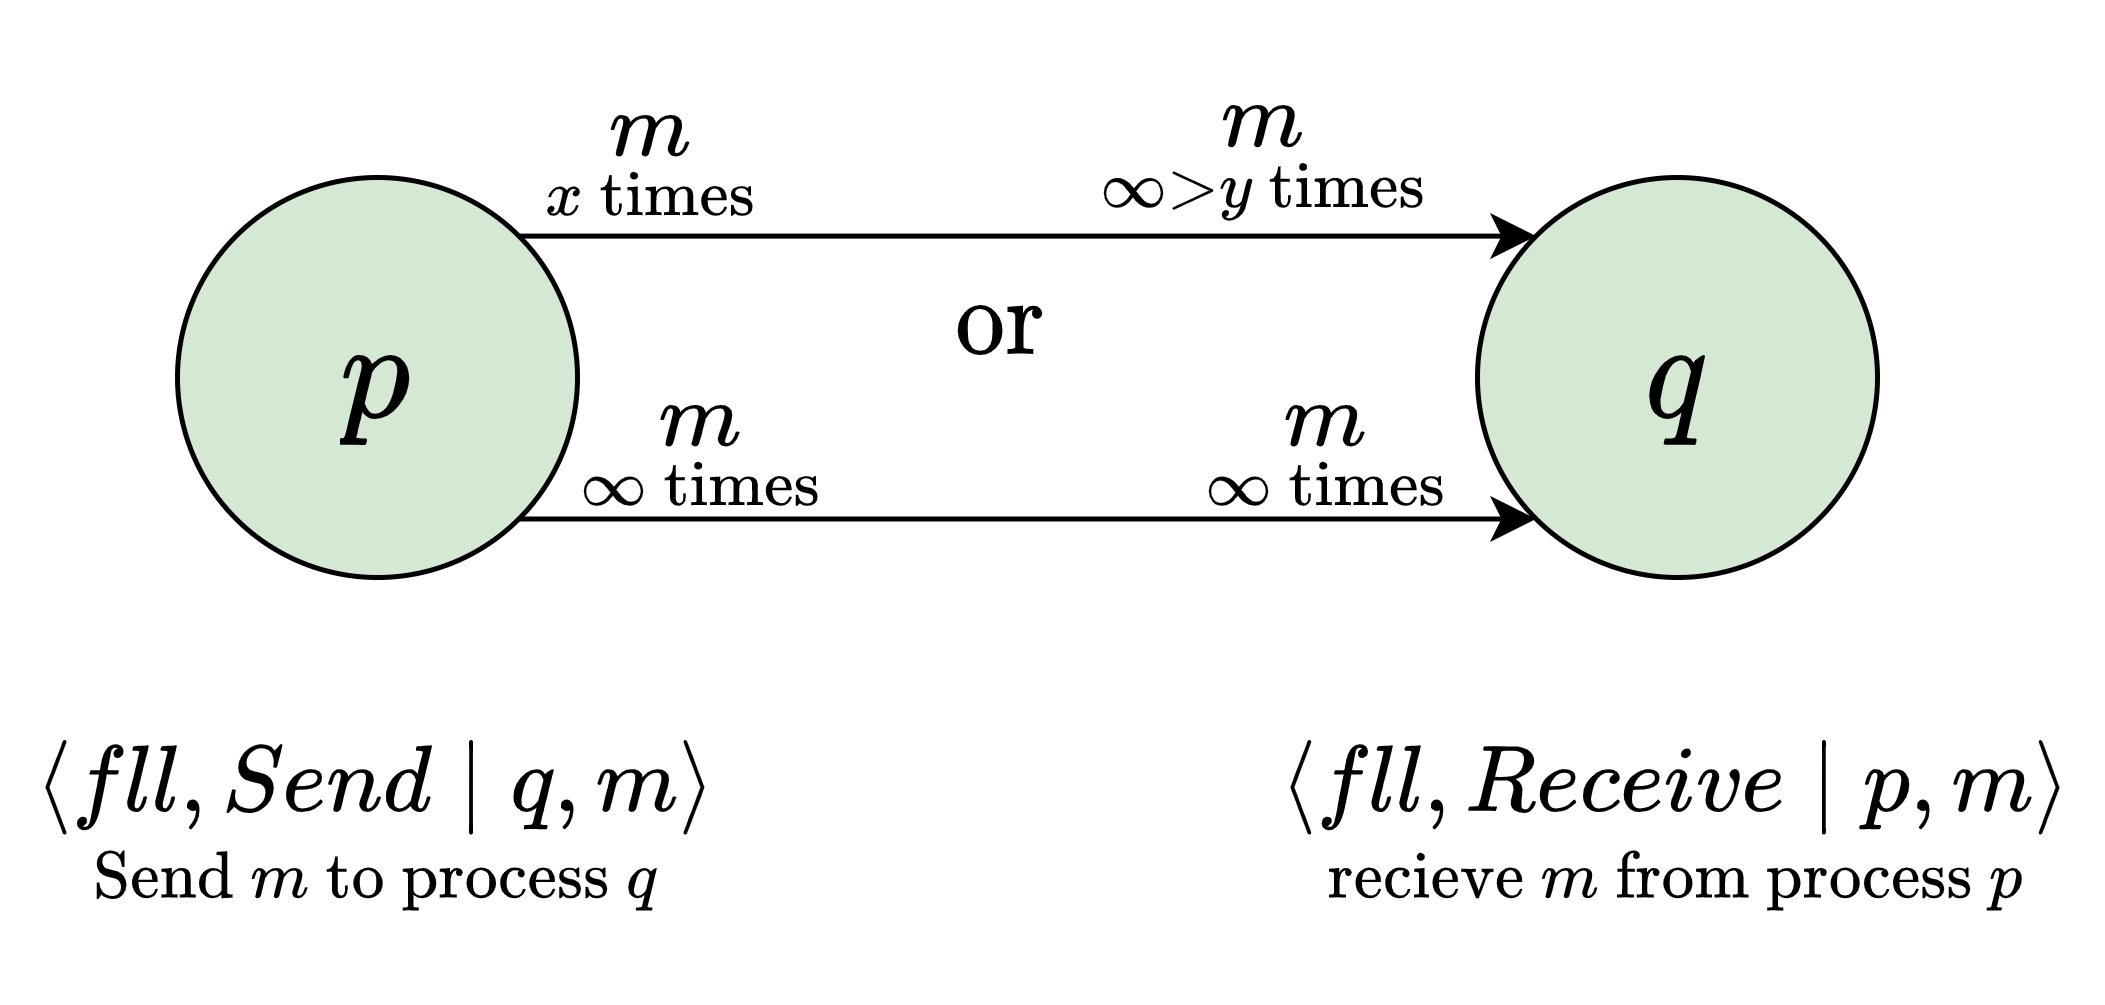
\includegraphics[width=.6\textwidth]{broadcast/images/fair_loss_links.drawio.png}
    \end{center}
    \begin{tabular}{l l p{.6\textwidth}}
        \textbf{Fair-Loss} & Liveness & Correct process $p$ infinitely sends message $m$ to correct process $q$ $\Rightarrow$ $q$ receives $m$ from $p$ infinitely many times. \\
        \textbf{Finite Duplication} & Liveness & Correct process $p$ sends message $m$ a finite number of times to $q$ $\Rightarrow$ $m$ cannot be received infinitely many times from $p$. \\
        \textbf{No Creation} & Safety & Some process $q$ receives a message $m$ with sender $p$ $\Rightarrow$ $p$ previously sent $m$ to $q$. \\
    \end{tabular}
\end{definitionbox}
\begin{definitionbox}{Stubborn Link}
    A link guaranteeing messages are received infinitely many times.
    \begin{center}
        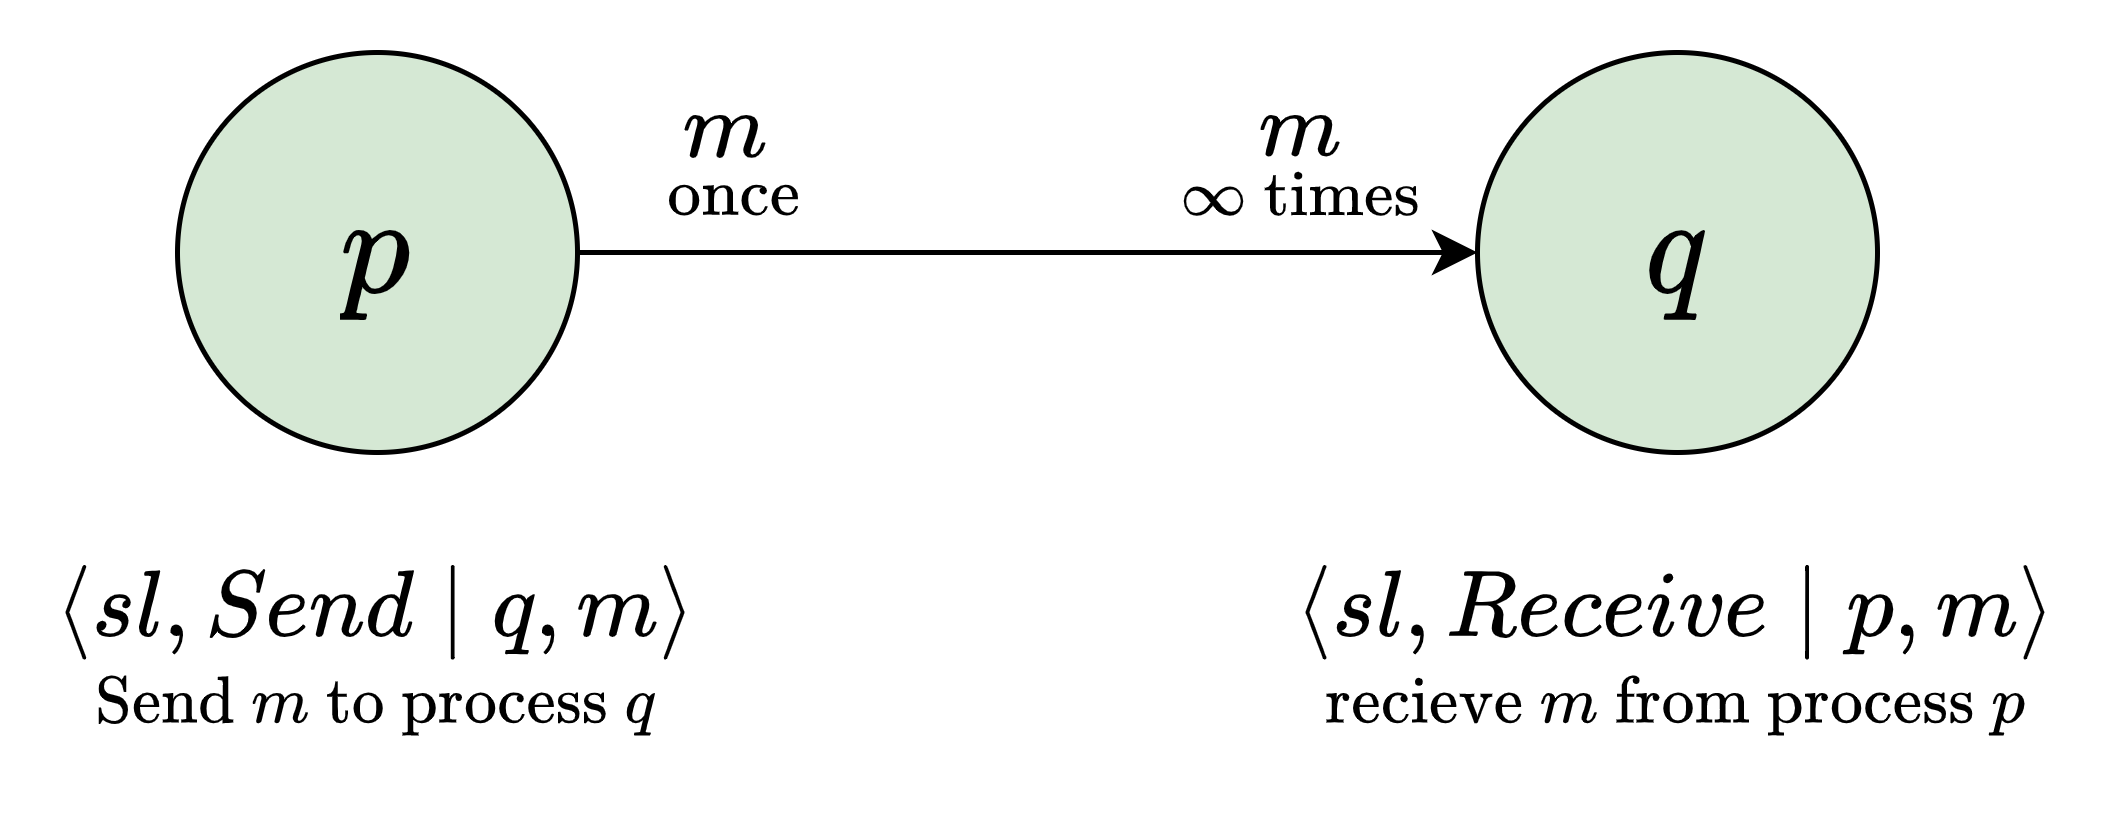
\includegraphics[width=.6\textwidth]{broadcast/images/stubborn_links.drawio.png}
    \end{center}
    \begin{center}
        \begin{tabular}{l l p{.6\textwidth}}
            \textbf{Stubborn Delivery} & Liveness & Correct process $p$ sends message $m$ to correct process $q$ $\Rightarrow$ $q$ receives $m$ from $p$ infinitely many times. \\
            \textbf{No Creation} & Safety & Some process $q$ receives a message $m$ with sender $p$ $\Rightarrow$ $p$ previously sent $m$ to $q$. \\
        \end{tabular}
    \end{center}
\end{definitionbox}

\begin{examplebox}{No change in mind}
    Implement stubborn links with elixir using the fair loss link.
    \tcblower
    \unfinished
\end{examplebox}

\begin{definitionbox}{Perfect Point-to-Point Link}
    \begin{center}
        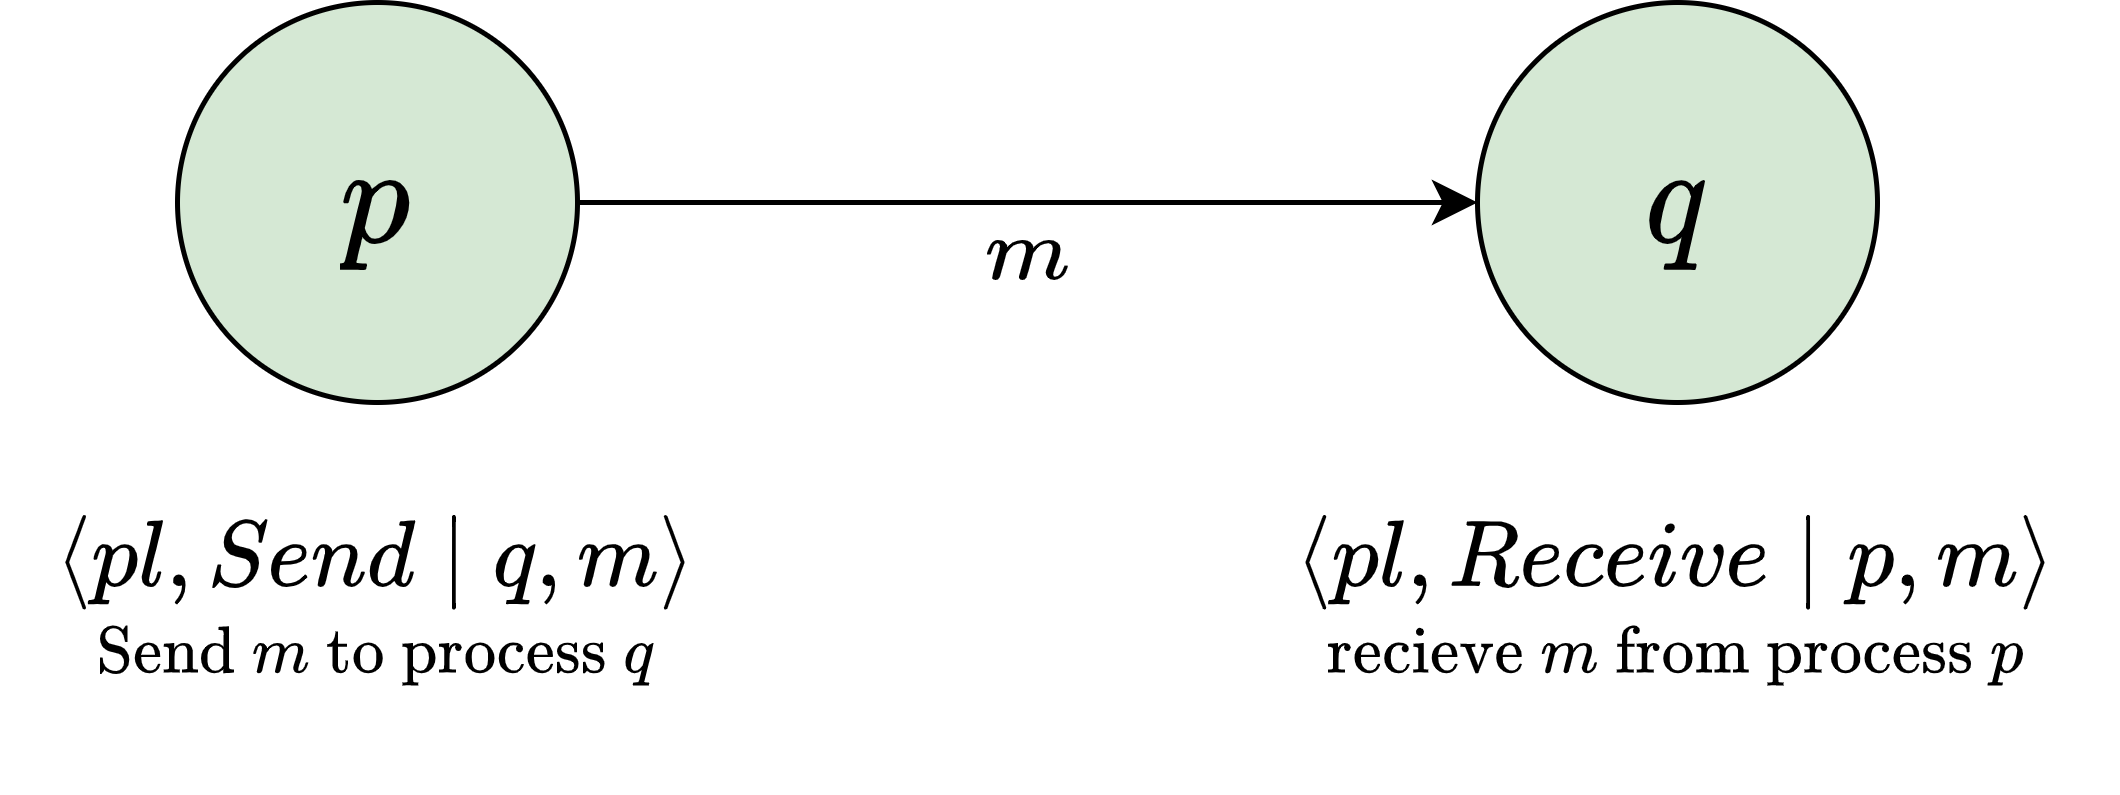
\includegraphics[width=.6\textwidth]{broadcast/images/perfect_links.drawio.png}
    \end{center}
    \begin{itemize}
        \item Also called \textit{reliable message passing}
    \end{itemize}
    \begin{center}
        \begin{tabular}{l l p{.6\textwidth}}
            \textbf{Reliable Delivery} & Liveness & Correct process $p$ sends $m$ to correct process $q$ $\Rightarrow$ $q$ will eventually receive $m$. \\
            \textbf{No Duplication} & Safety & No message is received by a process more than once. \\
            \textbf{No Creation} & Safety & Some process $q$ receives a message $m$ with sender $p$ $\Rightarrow$ $p$ previously sent $m$ to $q$. \\
        \end{tabular}
    \end{center}
\end{definitionbox}

\section{Failure Detection}
A failure detector provides a process with a list of \textit{suspected processes}.
\begin{itemize}
  \item Failure detectors make, and encapsulate some timing assumptions in order to determine which processes are suspect.
  \item They are not fully accurate, and their specification allows for this.
\end{itemize}

\begin{definitionbox}{Perfect Failure Detector}
  A failure detector that is never incorrect / is entirely accurate.
  \begin{itemize}
    \item Never changes its view on failure $\to$ once detected as crashed it cannot be \textit{unsuspected}.
    \item Often represented as $\mathcal{P}$
  \end{itemize}
  \begin{center}
    \begin{tabular}{l l p{.6\textwidth}}
      \textbf{Strong Completeness} & Liveness & Eventually every process that crashes is permanently detected as crashed by every correct process. \\
      \textbf{Strong Accuracy} & Safety & $p$ detected $\Rightarrow$ $p$ has crashed. No process is suspected before it crashed. \\
    \end{tabular}
\end{center}
\end{definitionbox}

We can implement a failure detector using timeouts and a heartbeat.
\begin{itemize}
  \item Perfect links used to send requests for heartbeat.
  \item If reply is not received before timeout, the process is suspected to have crashed.
  \item \textbf{perfect links} are only reliable for correct processes.
  \item Timeout period has to be long enough to send the heartbeat to all processes and for the receiving processes to respond. 
\end{itemize} 
\inputminted{elixir}{broadcast/code/perfect_failure_detector.ex}

This implementation meets the properties of a \textit{perfect failure detector} as:
\begin{center}
  \begin{tabular}{l p{.8\textwidth}}
    \textbf{Strong Completeness} & {If a process crashes it will no longer reply to heartbeat messages, 
    hence by \textit{perfect links} \textbf{no-creation} property, no correct process will receive 
    a heartbeat. So every correct process will detect a crash. } \\
    \textbf{Strong Accuracy} & A process can only miss the timeout if it has crashed under out timing assumption.
  \end{tabular}
\end{center}

\begin{definitionbox}{Eventually Perfect Failure Detector}
  A failure detector that is not entirely accurate.
  \begin{itemize}
    \item Can restore processes (no longer suspected).
    \item Often represented as $ \lozenge  \mathcal{P}$
  \end{itemize}
  \begin{center}
    \begin{tabular}{l l p{.6\textwidth}}
      \textbf{Strong Completeness} & Liveness & Eventually every process that crashes is permanently detected as crashed by every correct process.  \\
      \textbf{Eventual Strong Accuracy} & Liveness & Eventually no correct process is suspected by any other correct process \\
    \end{tabular}
\end{center}
\end{definitionbox}

\section{Best Effort Broadcast}
\begin{definitionbox}{Best Effort Broadcast / BEB}
    A non-reliable, single-shot broadcast.
    \begin{itemize}
        \item Only reliable if the broadcasting process is correct during broadcast (if crashing during broadcast only some messages may be delivered, and processes may disagree on delivery)
        \item No delivery agreement guarantee (correct processes may disagree on delivery)
        \item Uses \textit{Perfect Point-to-Point Link} and inherits properties from it.
    \end{itemize} 
    \begin{center}
        \begin{tabular}{l l p{.6\textwidth}}
            \textbf{Validity} & Liveness & If a correct process broadcasts a message then every correct process eventually receives it. \\
            \textbf{No Duplication} & Safety & No message is received by a process more than once. \\
            \textbf{No Creation} & Safety & No broadcast is delivered unless it was broadcast. \\
        \end{tabular}
    \end{center}
\end{definitionbox}
We can implement this in elixir using the send and receive primitives as \textit{Perfect Point-to-Point Link}.

\inputminted{elixir}{broadcast/code/perfect_point_to_point_links.ex}

\section{Reliable Broadcast}
\begin{definitionbox}{Reliable Broadcast}
    Adds a delivery guarantee to \textit{best effort broadcast}  
    \begin{center}
        \begin{tabular}{l l p{.6\textwidth}}
            \textbf{Agreement} & Liveness & If a correct process delivers message $m$ then all correct processes deliver $m$ \\
            \multicolumn{3}{c}{\textbf{All Properties from Best Effort Broadcast}} \\
        \end{tabular}
    \end{center}
    \begin{itemize}
        \item The combination of \textbf{Validity} and \textbf{Agreement} form a \textit{termination property} (system reaches agreement in finite time).
        \item Correct processes agree on messages delivered even if the broadcaster crashes while sending.
    \end{itemize}
\end{definitionbox}
\begin{center}
    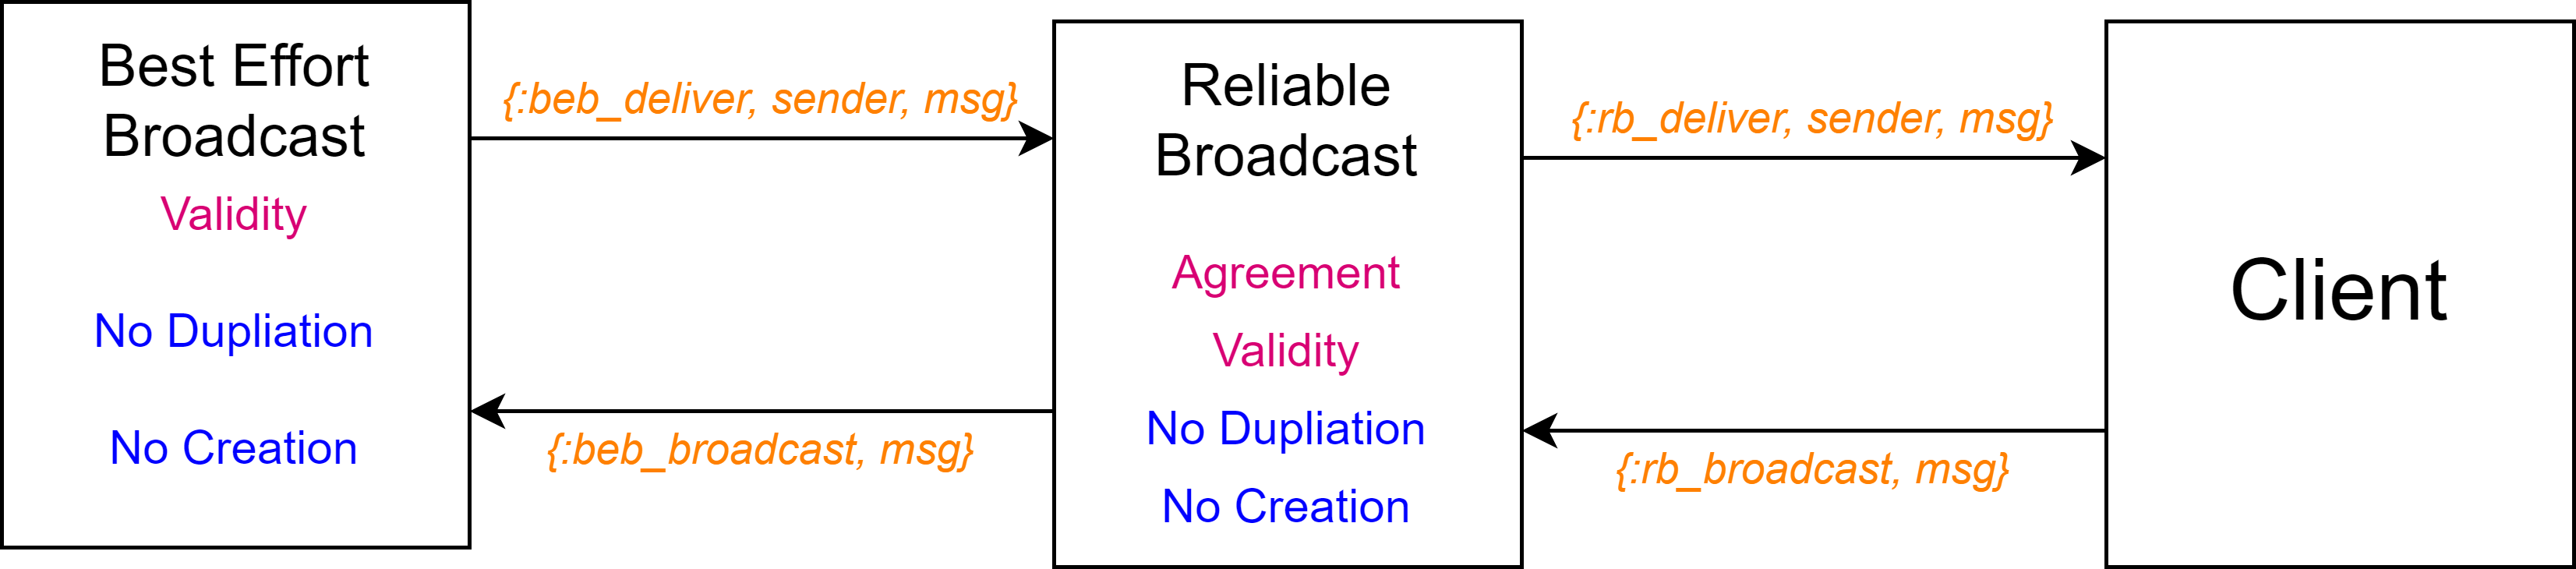
\includegraphics[width=.8\textwidth]{broadcast/images/reliable_broadcast.drawio.png}
  \end{center}


\subsection{Eagre Reliable Broadcast}
\begin{definitionbox}{Eagre Reliable Broadcast}
    A \textit{reliable broadcast} where every process re-broadcasts every message it delivers.
    \begin{itemize}
        \item If the broadcasting process crashes, and only some correct processes deliver the message, then re-broadcast ensures eventually all will receive.
        \item This broadcast is \textit{fail-silent}
        \item Very inefficient to implement, broadcast to $n$ processes results in $O(n^2)$ messages from $O(n)$ \textit{BEB} broadcasts.
        \item \textbf{Validity} property combined with retransmission provides \textbf{agreement}.
    \end{itemize}
    \begin{center}
        \begin{tabular}{l l p{.6\textwidth}}
            \multicolumn{3}{c}{\textbf{All Properties from Reliable Broadcast}} \\
        \end{tabular}
    \end{center}
\end{definitionbox}

\inputminted{elixir}{broadcast/code/eagre_reliable_broadcast.ex}

\subsection{Lazy Reliable Broadcast}
\begin{definitionbox}{Lazy Reliable Broadcast}
    A \textit{reliable broadcast} using \textit{Best Effort Broadcast} with a \textit{Failure Detector} to enforce agreement.
    \begin{itemize}
        \item Uses a \textit{perfect failure detector}.
        \item When a process is detected to have crashed, all broadcasts delivered from the process are rebroadcasted
        \item Agreement is derived from the \textbf{validity} of \textit{best effort broadcast}, that every correct process broadcasts every message delivered from a crashed process and the properties of the \textit{perfect failure detector}.
    \end{itemize}
\end{definitionbox}

\begin{center}
  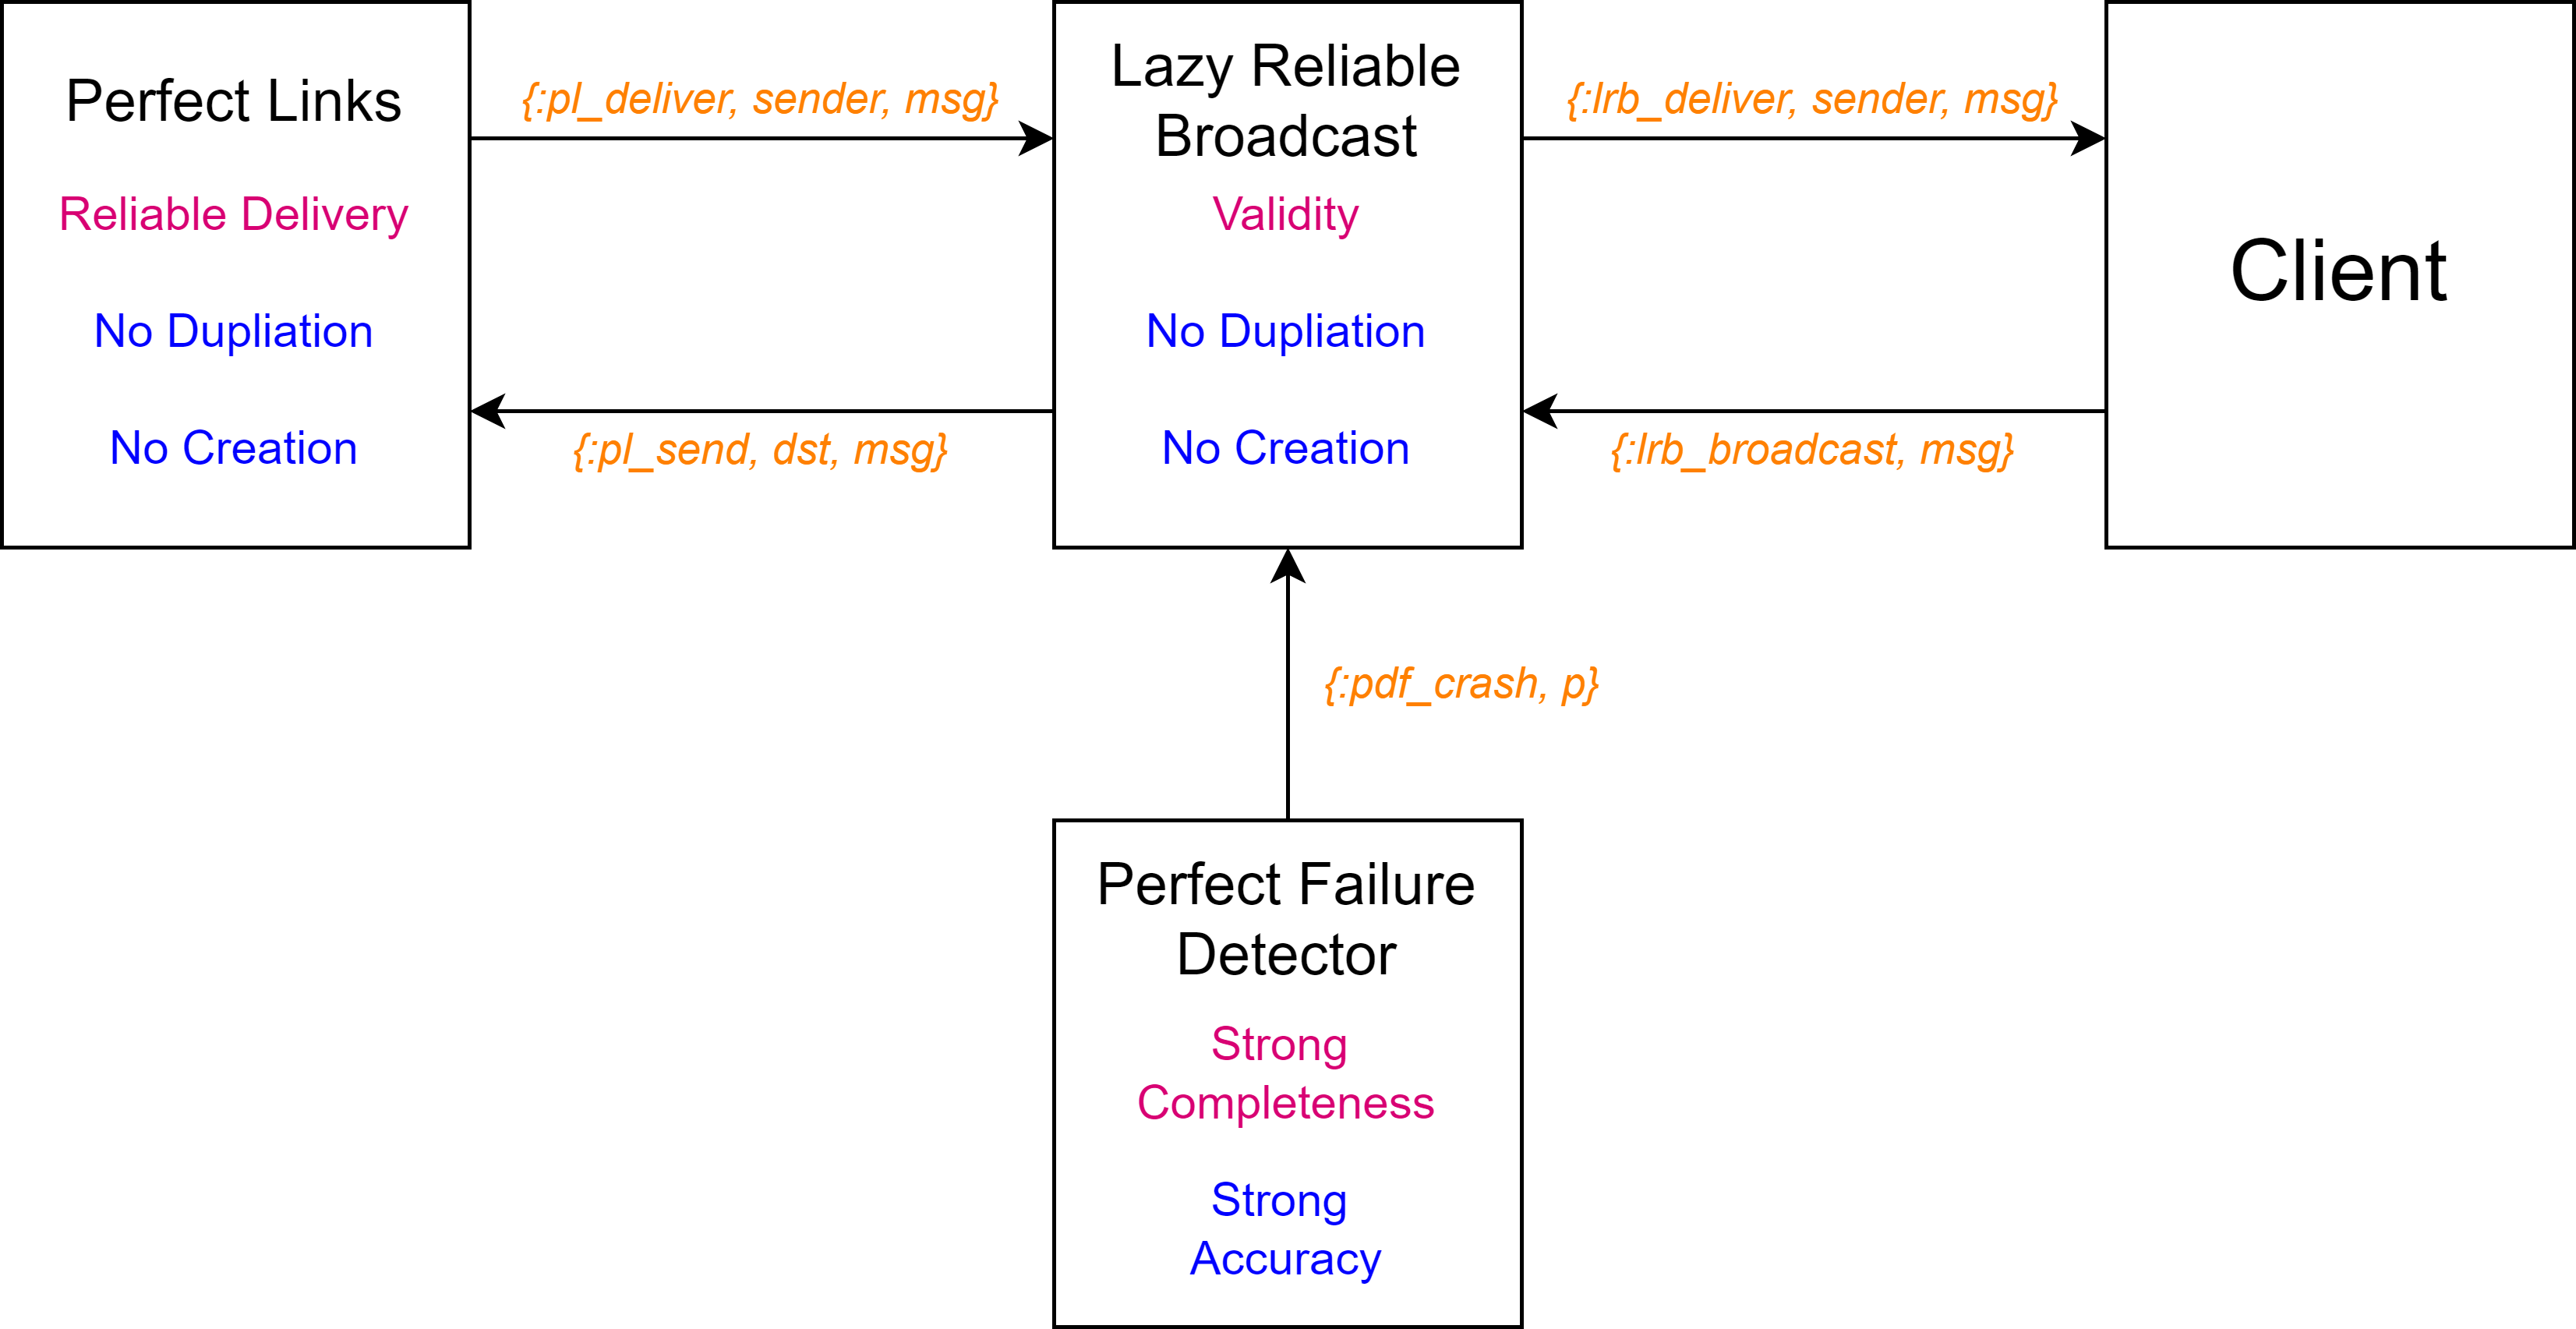
\includegraphics[width=.8\textwidth]{broadcast/images/lazy_reliable_broadcast.drawio.png}
\end{center}

\inputminted{elixir}{broadcast/code/lazy_reliable_broadcast.ex}

\subsection{Uniform Reliable Broadcast}
\begin{definitionbox}{Uniform Reliable Broadcast / URB}
    \begin{center}
        \begin{tabular}{l l p{.6\textwidth}}
            \textbf{Uniform Agreement} & Liveness & If a process delivers a message, then all correct processes will deliver the message. \\
            \multicolumn{3}{c}{\textbf{All Properties from Best Effort Broadcast}} \\
        \end{tabular}
    \end{center}
    \begin{itemize}
        \item Implies that faulty processes deliver a subset of messages delivered to correct processes (stronger than \textbf{agreement} - only for correct processes).
        \item Avoids any scenario where a crashed process broadcasts and only a crashed process delivers (correct processes miss message).
    \end{itemize}
\end{definitionbox}
\begin{center}
    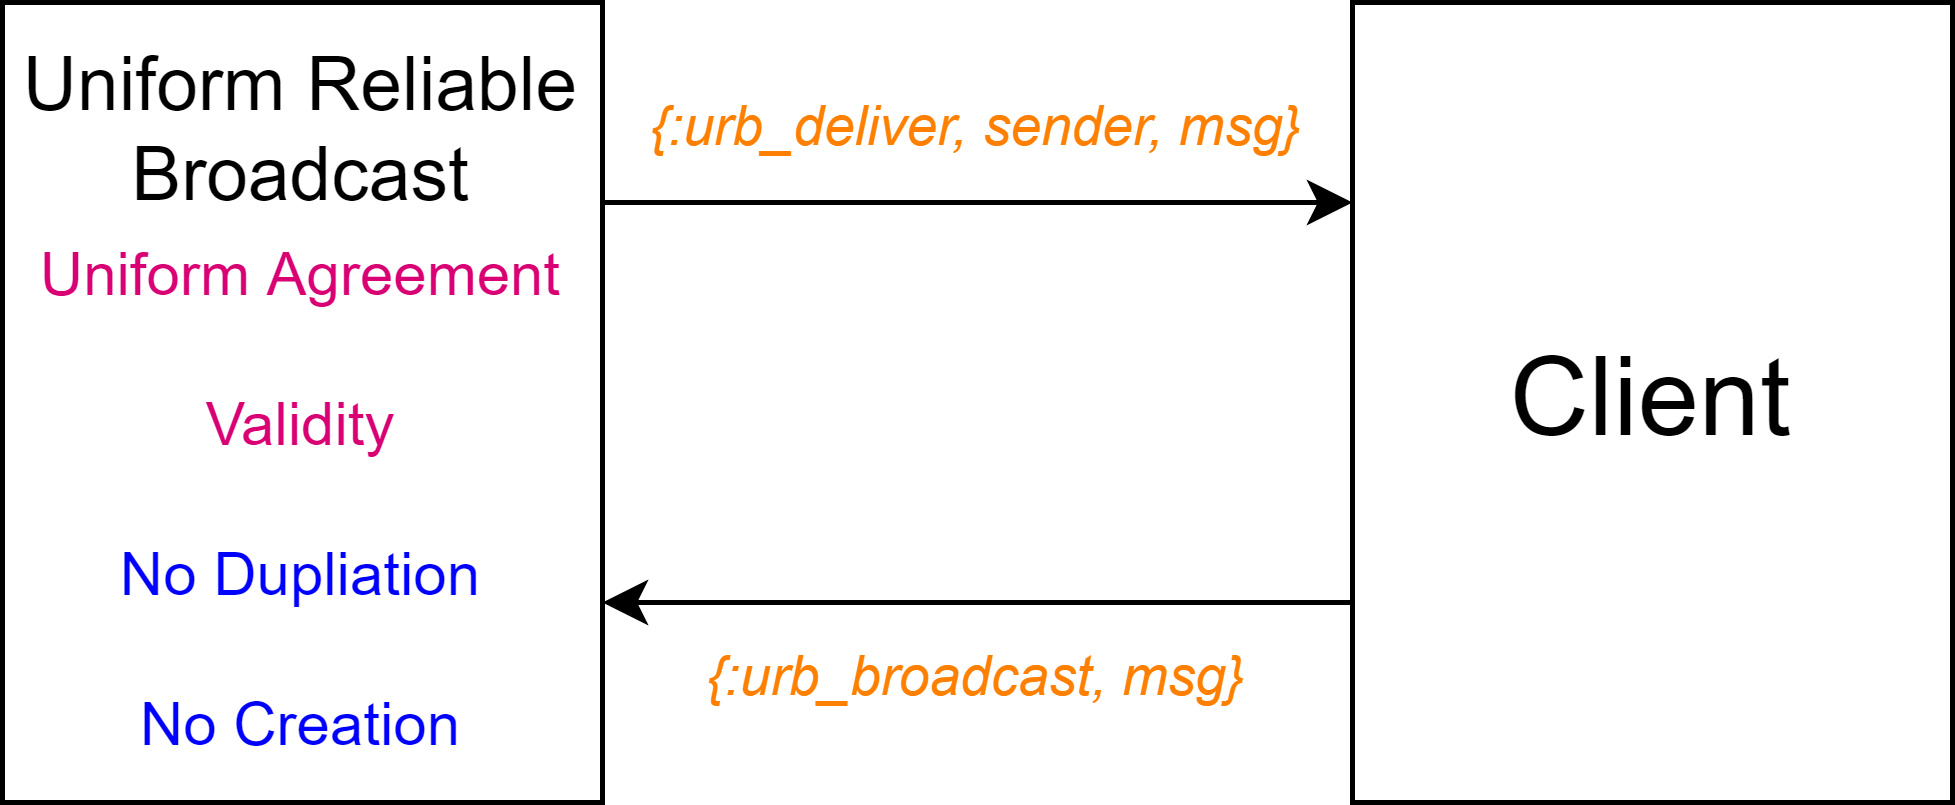
\includegraphics[width=.5\textwidth]{broadcast/images/uniform_reliable_broadcast.drawio.png}
\end{center}

\begin{definitionbox}{Majority Ack Uniform Reliable Broadcast}
    A \textit{uniform reliable broadcast} implementation that assumes a majority of processes are correct.
    \begin{itemize}
        \item \textit{Fail-silent} and does not use a \textit{failure detector}.
        \item If $n$ processes may crash, then $2n+1$ processes are needed with at least $n+1$ (majority) being correct
    \end{itemize}
\end{definitionbox}
\begin{center}
    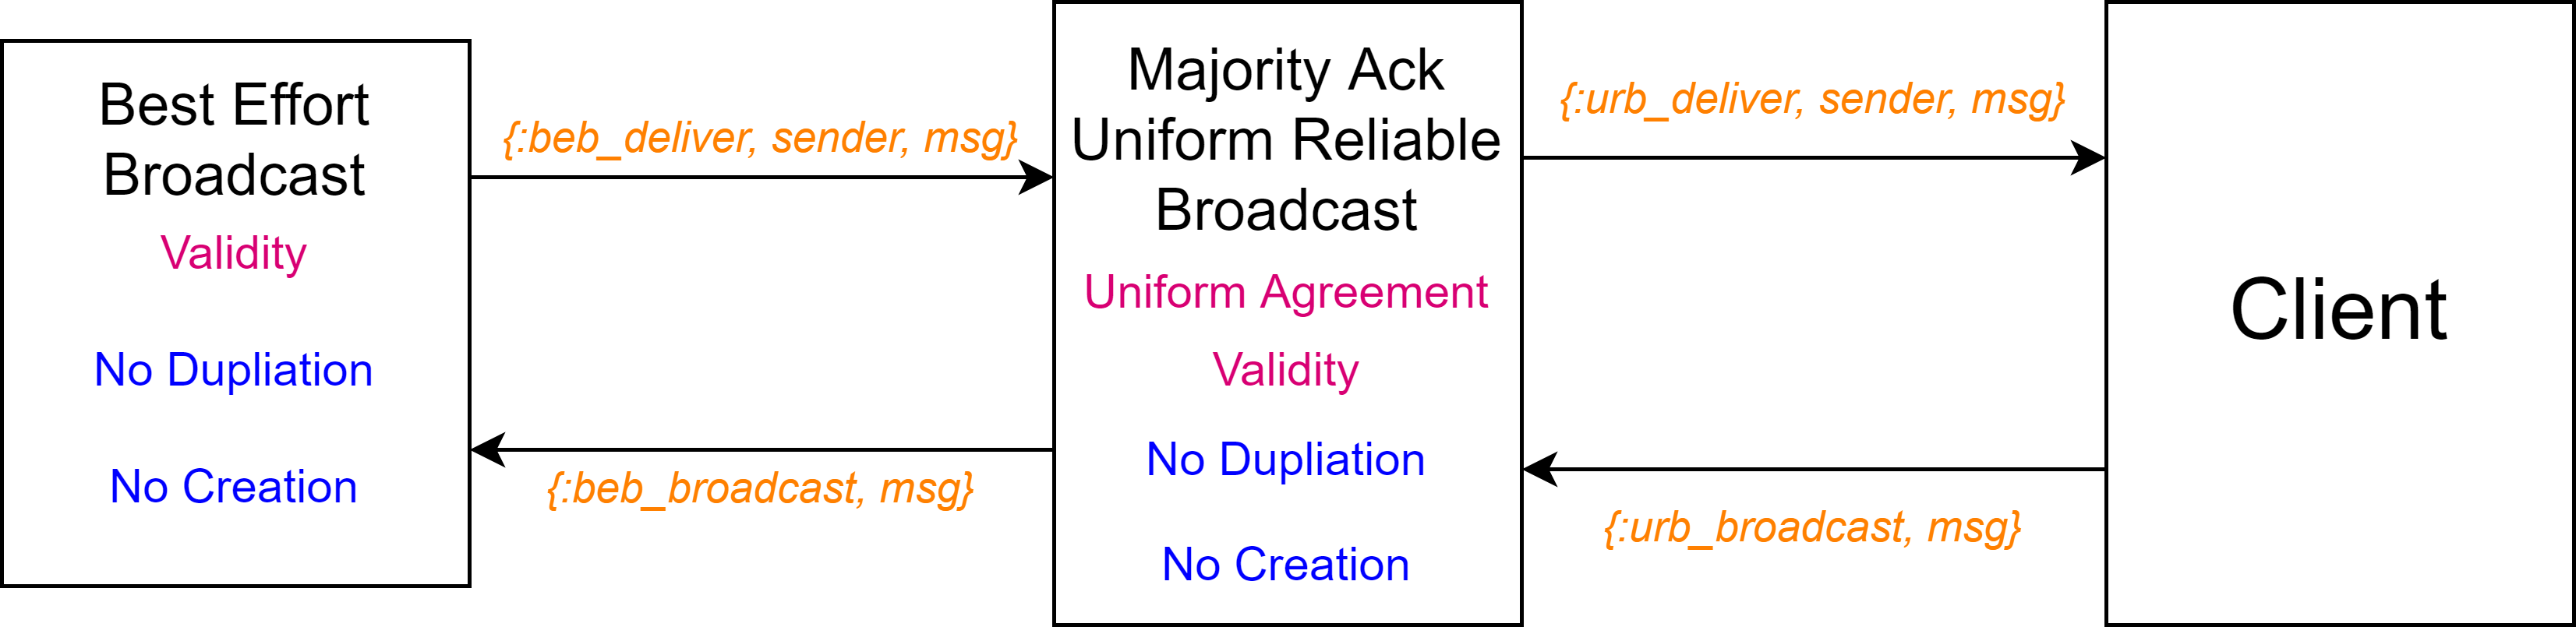
\includegraphics[width=.8\textwidth]{broadcast/images/majority_ack_uniform_reliable_broadcast.drawio.png}
\end{center}
Each process tracks which other processes \textit{BEB} them a specific message. Once the majority have done this, then can \textit{URB} deliver the message.
\begin{center}
    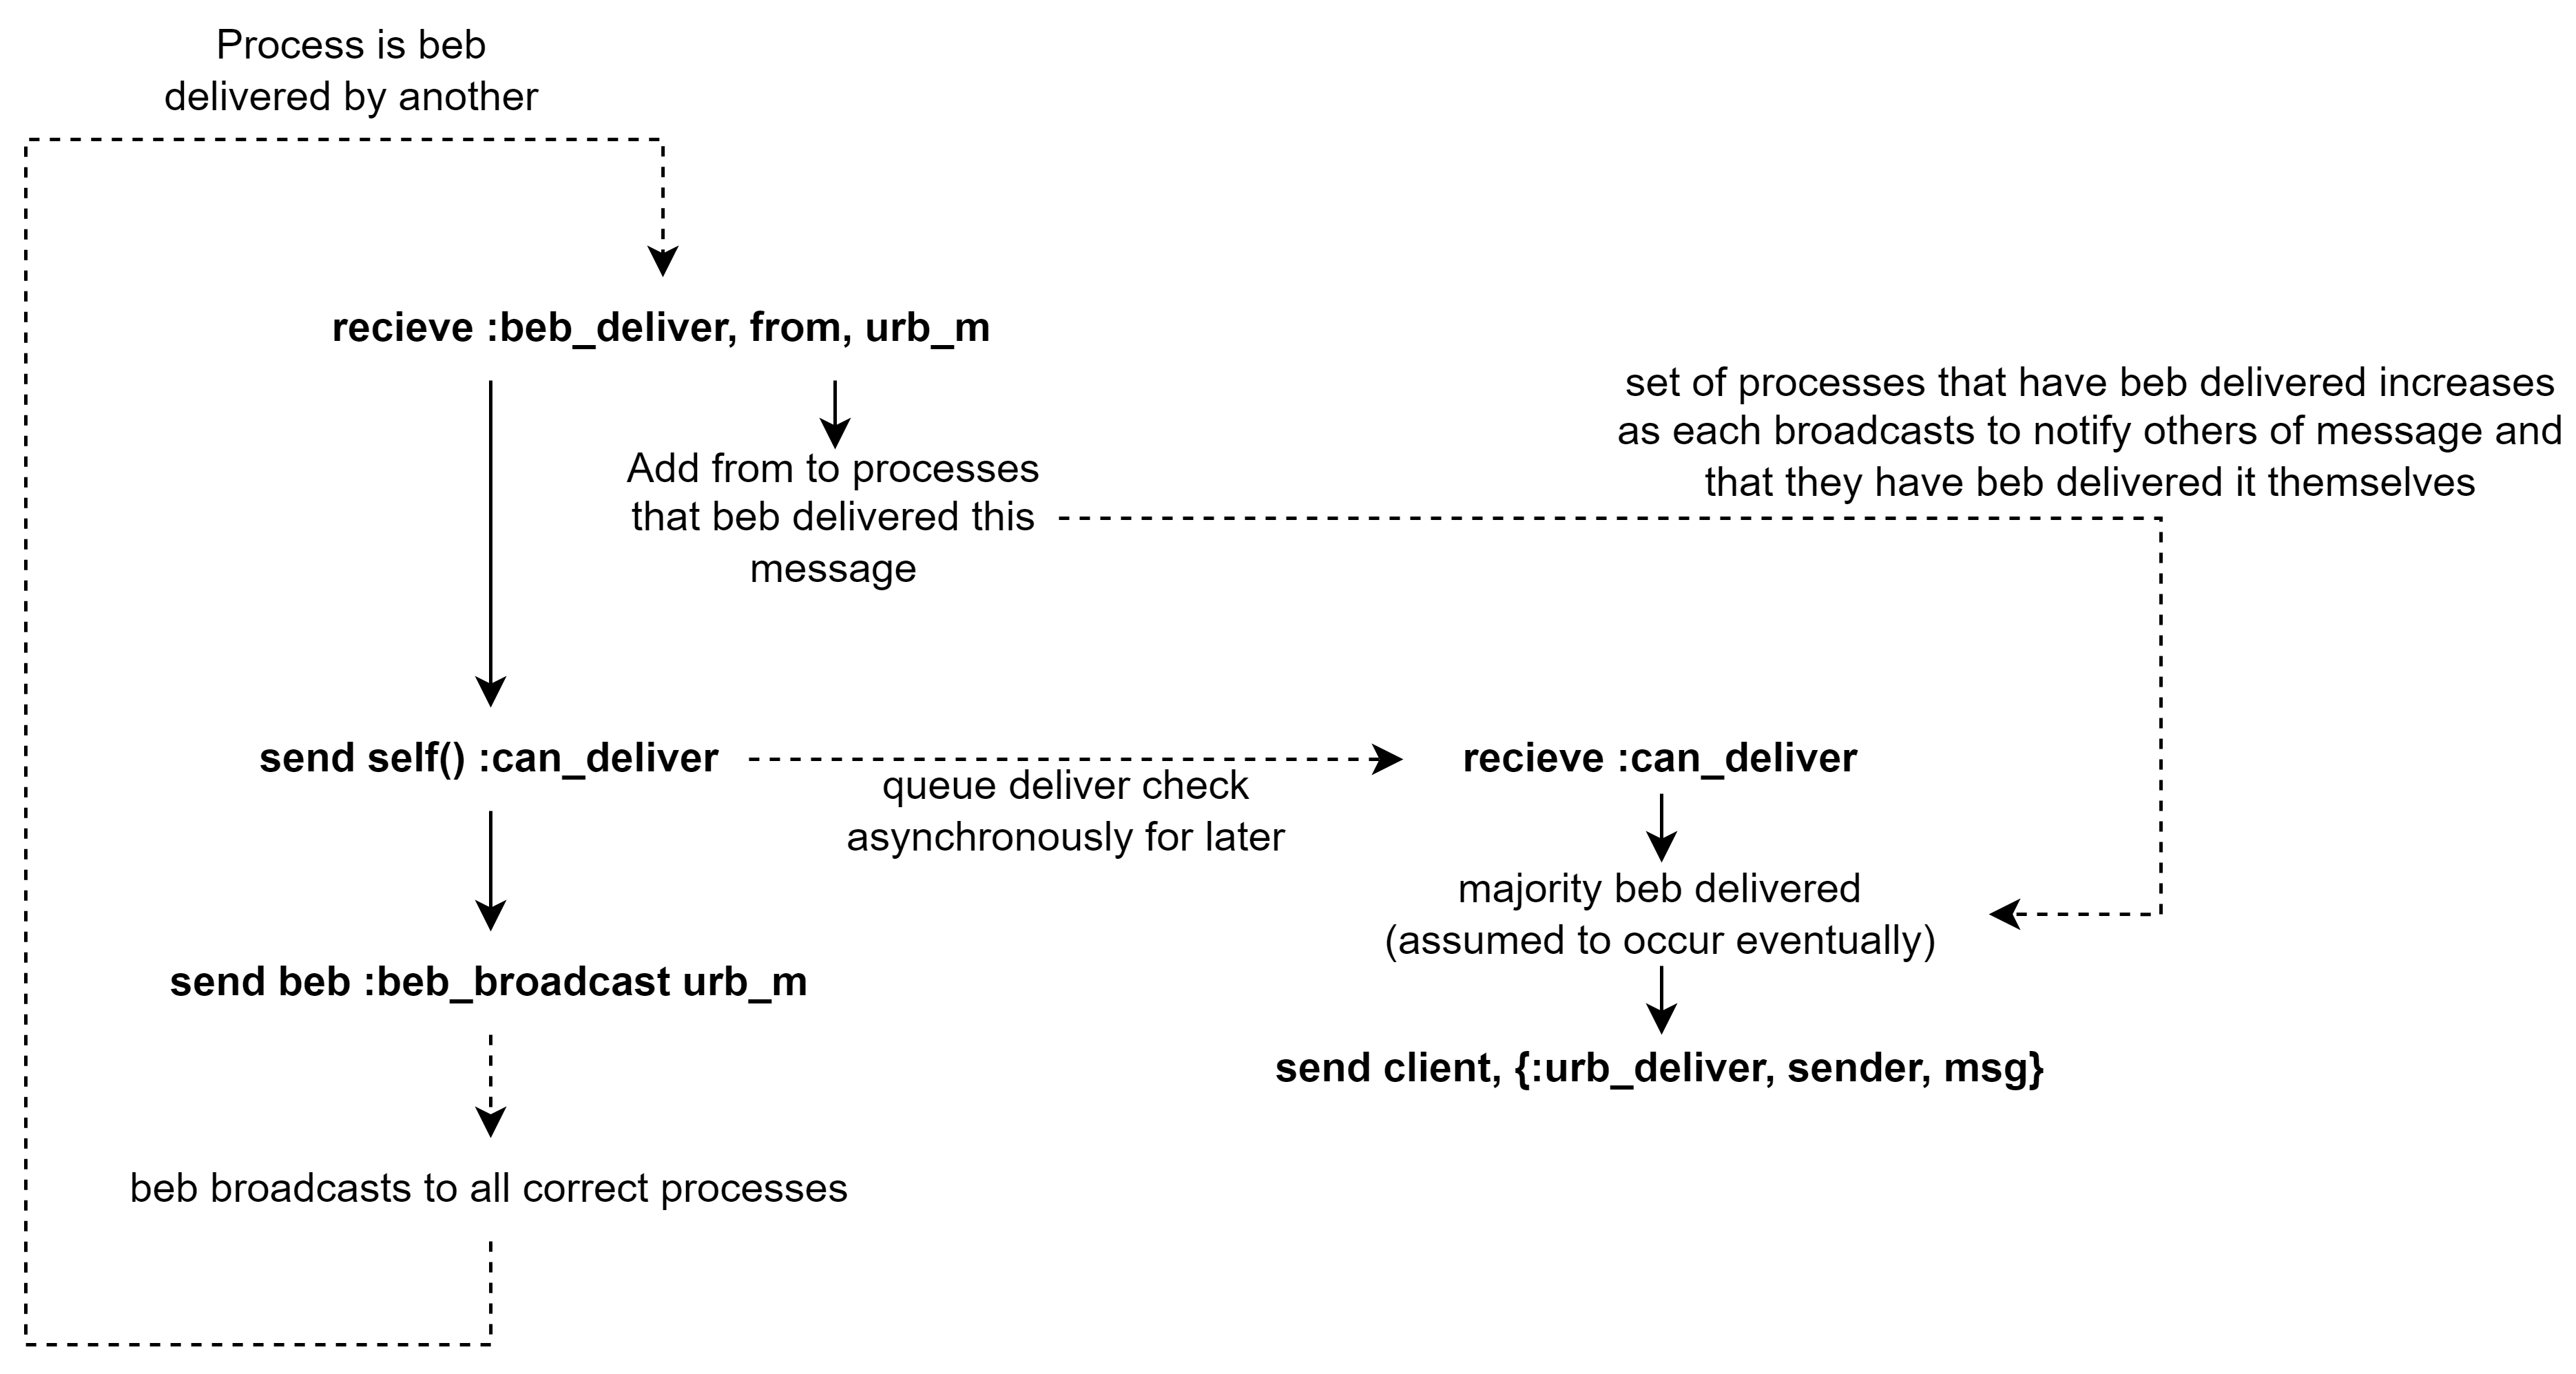
\includegraphics[width=.8\textwidth]{broadcast/images/majority_ack_urb_correctness.drawio.png}
\end{center}
\begin{center}
    \begin{tabular}{l p{.8\textwidth}}
        \textbf{No Creation} & Provided by \textit{BEB}. \\
        \textbf{No Duplication} & Messages delivered are tracked in a \mintinline{elixir}{delivered} set. \\
        \textbf{Validity} & As a \textit{URB} sends via \textit{BEB} (valid), and all messages \textit{BEB} are eventually \textit{URB} delivered. \\
        \textbf{Uniform Agreement} & If correct process $Q$ \textit{URB} delivers a message $M$, then $Q$ was \textit{BEB} delivered by a majority of 
        processes (assumed correct), which means at least $1$ correct process \textit{BEB} broadcast $M$. Hence all correct processes eventually \textit{BEB} deliver (and then \textit{URB} deliver) $M$. \\
    \end{tabular}
\end{center}
\inputminted{elixir}{broadcast/code/majority_ack_uniform_reliable_broadcast.ex}

\subsection{Process Configuration}
\begin{center}
    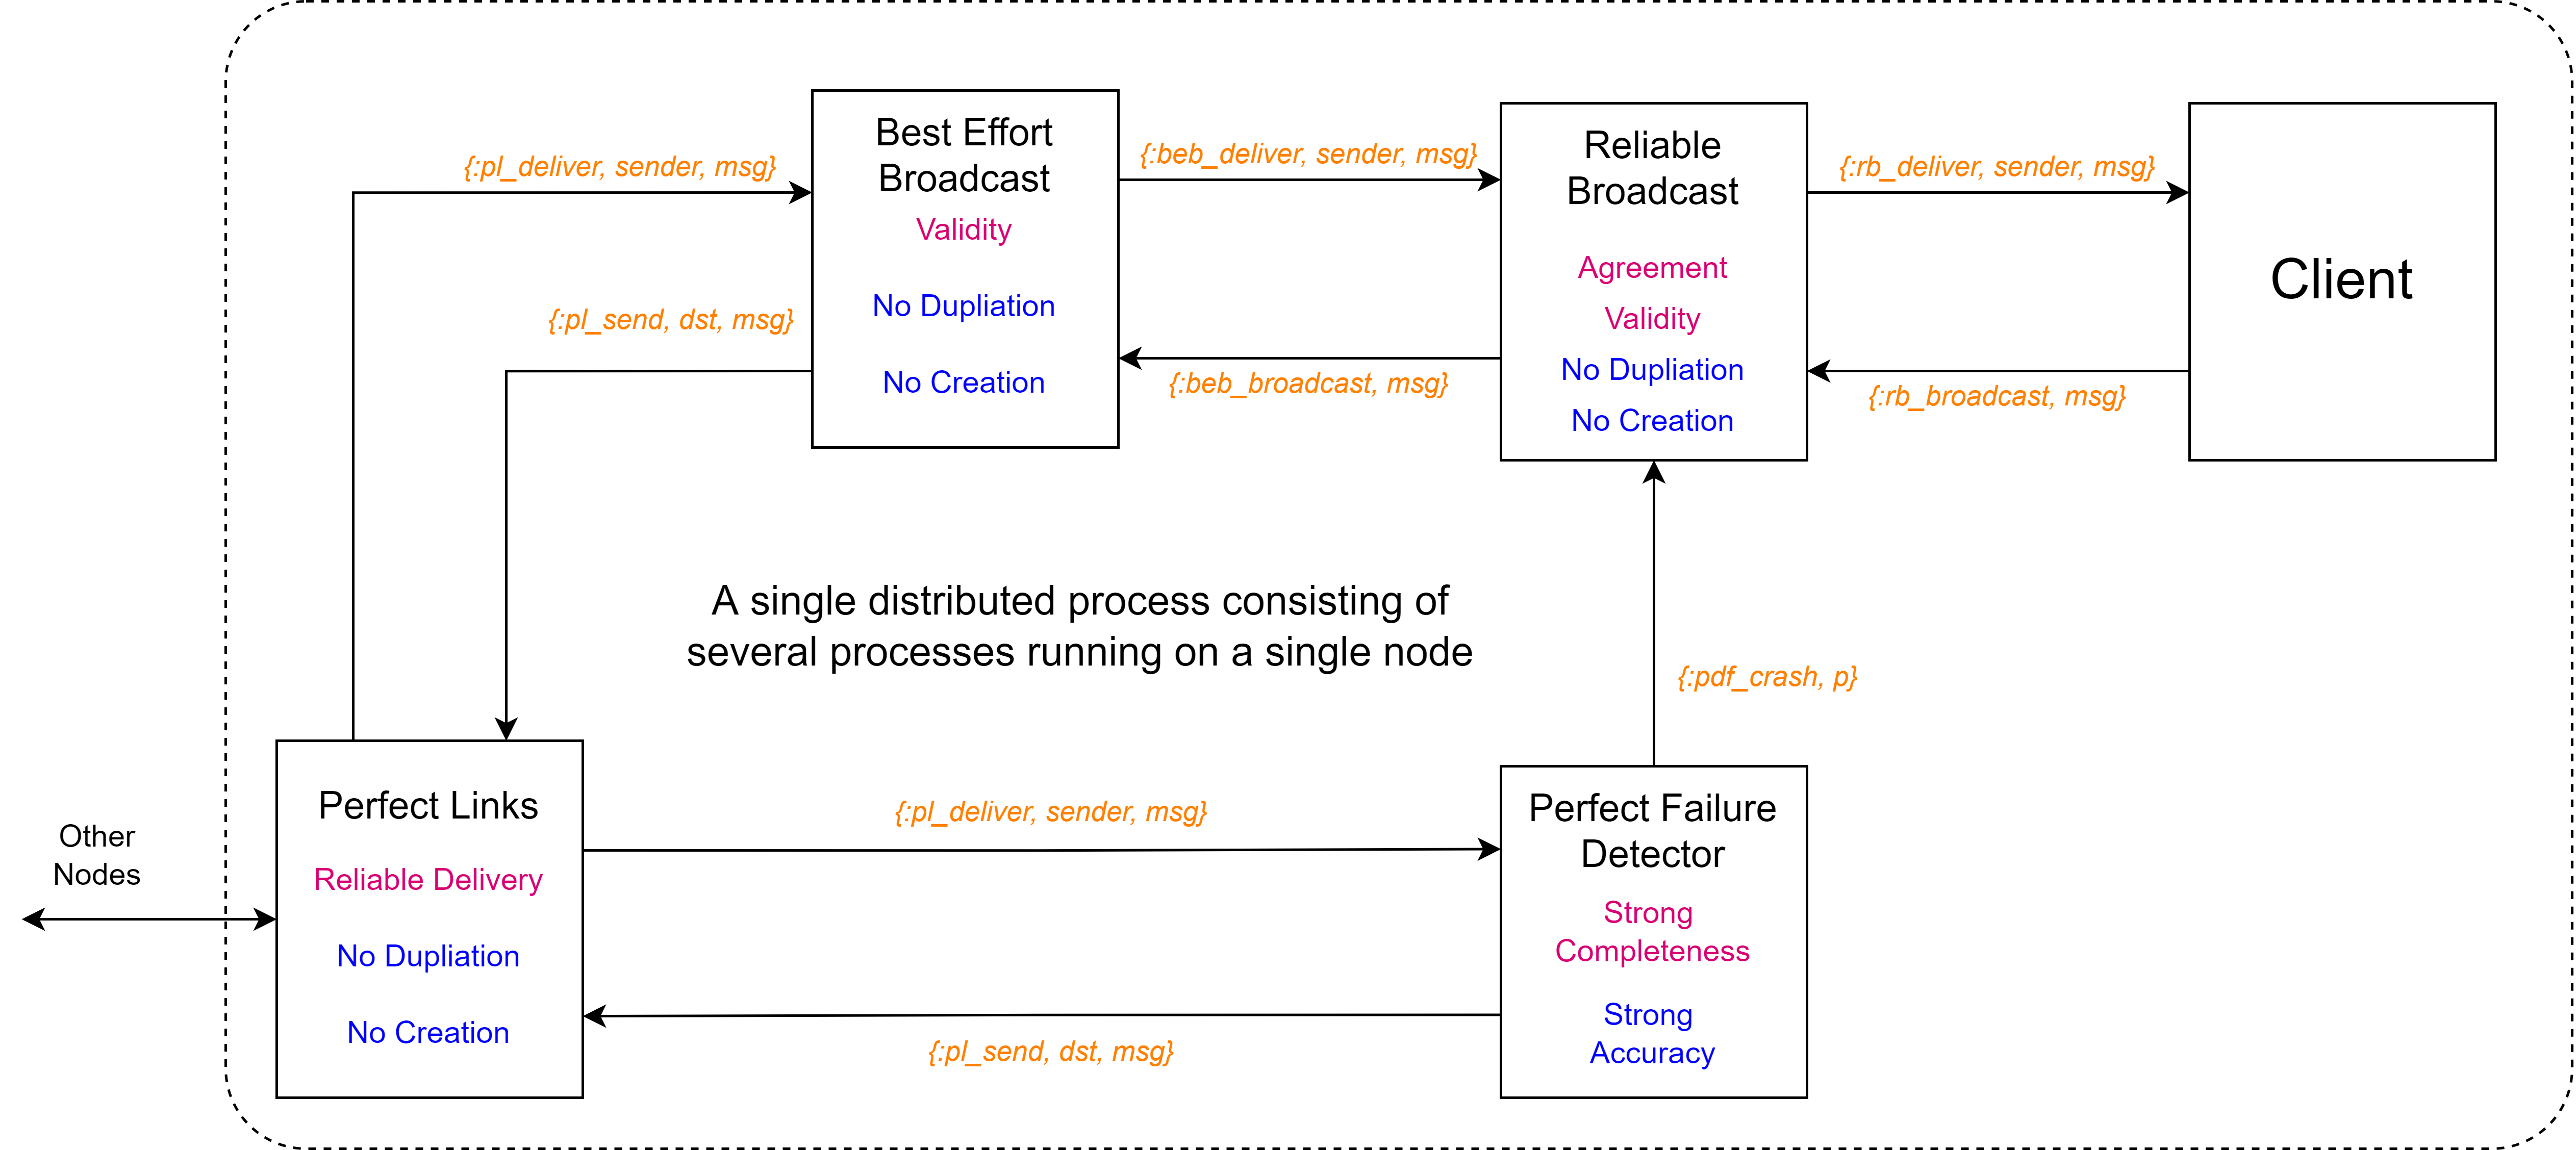
\includegraphics[width=\textwidth]{broadcast/images/process_config.drawio.png}
\end{center}


\section{Message Ordering}
\subsection{FIFO Message Delivery}
\begin{definitionbox}{First In First Out/FIFO Reliable Broadcast (FRB)}
    Messages delivered in broadcast order.
    \begin{center}
        \begin{tabular}{l l p{.6\textwidth}}
            \textbf{FIFO Delivery} & Safety & If a process broadcasts $M_1 \prec M_2$ then all correct processes will deliver $M_1 \prec M_2$. \\
            \multicolumn{3}{c}{\textbf{All Properties from Reliable Broadcast}} \\
        \end{tabular}
    \end{center}
    \begin{itemize}
        \item Only applies per-sender, this is analogous to sequential consistency in concurrency.
        \item The same scheme can be applied to \textit{uniform reliable broadcast} (\textit{FIFO-URB}).
        \item Same number of messages as the underlying reliable broadcast implementation.
    \end{itemize}
\end{definitionbox}
\begin{center}
    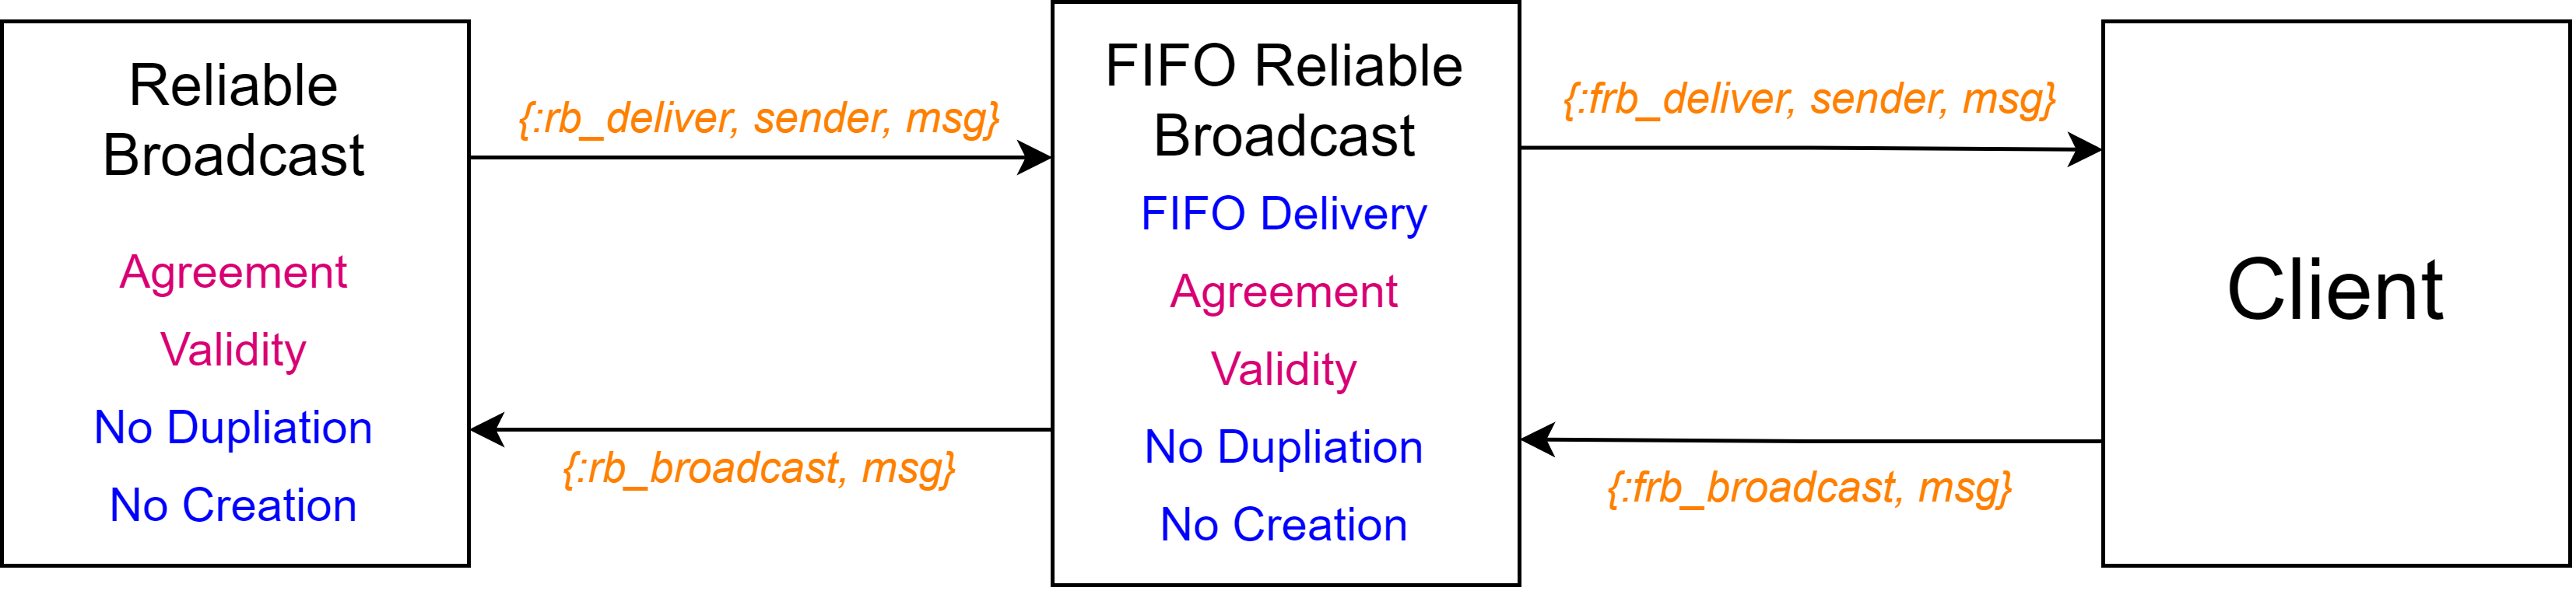
\includegraphics[width=.8\textwidth]{broadcast/images/fifo_reliable_broadcast.drawio.png}
\end{center}
\inputminted{elixir}{broadcast/code/fifo_reliable_broadcast.ex}

\subsection{Causal Order Message Delivery}
\begin{definitionbox}{Causal Order Relation}
    A relation over messages $M_1 \to M_2$ when $M_1$ causes $M_2$. A causal relation between messages is determined by:
    \begin{center}
        \begin{tabular}{l l l}
            \textbf{FIFO Order} & Process message broadcast order & $\{ \text{broadcast}, M_1 \} \prec \{\text{broadcast}, M_2 \} \Rightarrow M_1 \to M_2$. \\
            \textbf{Local Order} & Process delivers and then broadcasts & $\{\text{deliver}, M_1 \} \prec \{\text{broadcast}, M_2\}$ \\
            \textbf{Transitivity} & & $M_1 \to M_2 \land M_2 \to M_3 \Rightarrow M_1 \to M_3$ \\
        \end{tabular}
    \end{center}
\end{definitionbox}

\begin{definitionbox}{Causal Order/CO Message Delivery}
    Messages are delivered in an order respecting the causal order relation.
    \begin{center}
        \begin{tabular}{l l p{.6\textwidth}}
            \textbf{Causal Delivery Property} & Safety & If a process delivers message $M_2$, it must have already delivered every message $M_1$ such that $M_1 \to M_2$. \\
            \multicolumn{3}{c}{\textbf{All Properties from Uniform Reliable Broadcast}} \\
        \end{tabular}
    \end{center}
\end{definitionbox}
\begin{center}
    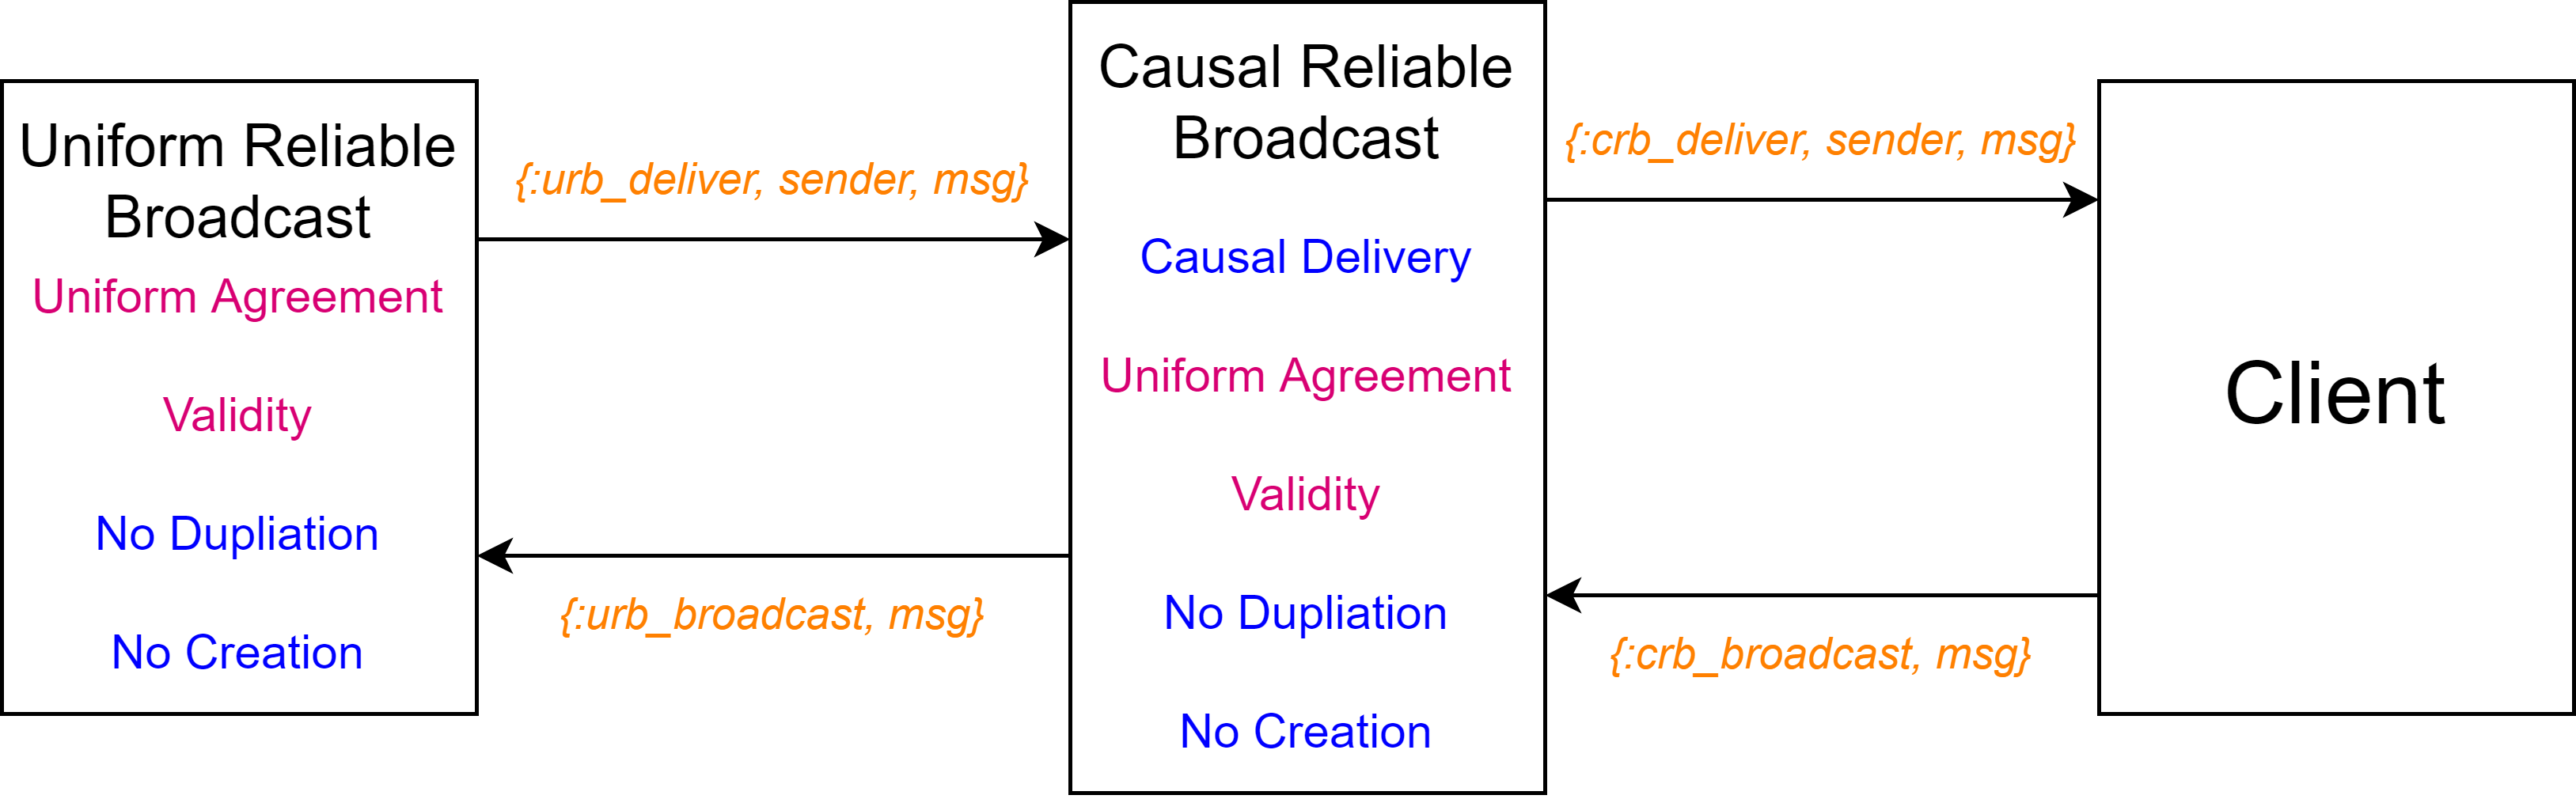
\includegraphics[width=.8\textwidth]{broadcast/images/causal_reliable_broadcast.drawio.png}
\end{center}
\subsubsection{No Wait Implementation}
One implementation of this spec if a \textit{causal reliable broadcast} that never waits. This is done by dropping any message that precedes the delivered message that has not already been delivered.
\begin{itemize}
    \item Each message has a list of past messages \mintinline{elixir}{m_past}
    \item The \mintinline{elixir}{m_past} contains all causally preceding messages as a bundle.
    \item Hence whenever \textit{URB} delivering a message all preceding messages are already available to \textit{CRB} deliver first.
\end{itemize}
\begin{center}
    \begin{tabular}{l p{.8\textwidth}}
        \textbf{Casual Delivery} & Ensured as each message contains all of its past messages which are \textit{CRB} delivered prior to the message. \\
        \multicolumn{2}{l}{\textbf{No Creation}, \textbf{No Duplication} and \textbf{Validity} from \textit{Uniform Reliable Broadcast}} \\
    \end{tabular}
\end{center}
Past will grow large over time as the set of preceding messages grows.
\begin{itemize}
    \item Large past uses up memory and network bandwidth
    \item Can selectively purge/garbage collect past messages (e.g when it is known a message recipient has already received some past messages)
\end{itemize}
\inputminted{elixir}{broadcast/code/causal_reliable_broadcast_no_wait.ex}

\subsubsection{Vector Clock Implementation}
\begin{sidenotebox}{Dynamic Deadlock Detection}
    Vector clocks can also be used in dynamically detecting data races in programs, as discussed in 60007 - Theory and practice of Concurrent Programming.
\end{sidenotebox}
\begin{itemize}
    \item Each process maintains a vector clock of (processes $\to$ messages \textit{CRB delivered}) and a count of messages that it has \textit{RB broadcast}.
    \item When sending a message, the  the vector clock and the \textit{RB Broadcasts} count are sent.
    \item A message is only delivered if the sender's vector clock is $\leq$ the receiver's vector clock (the current process has seen all the messages the sender had seen, when it sent this message)
\end{itemize}
\begin{center}
    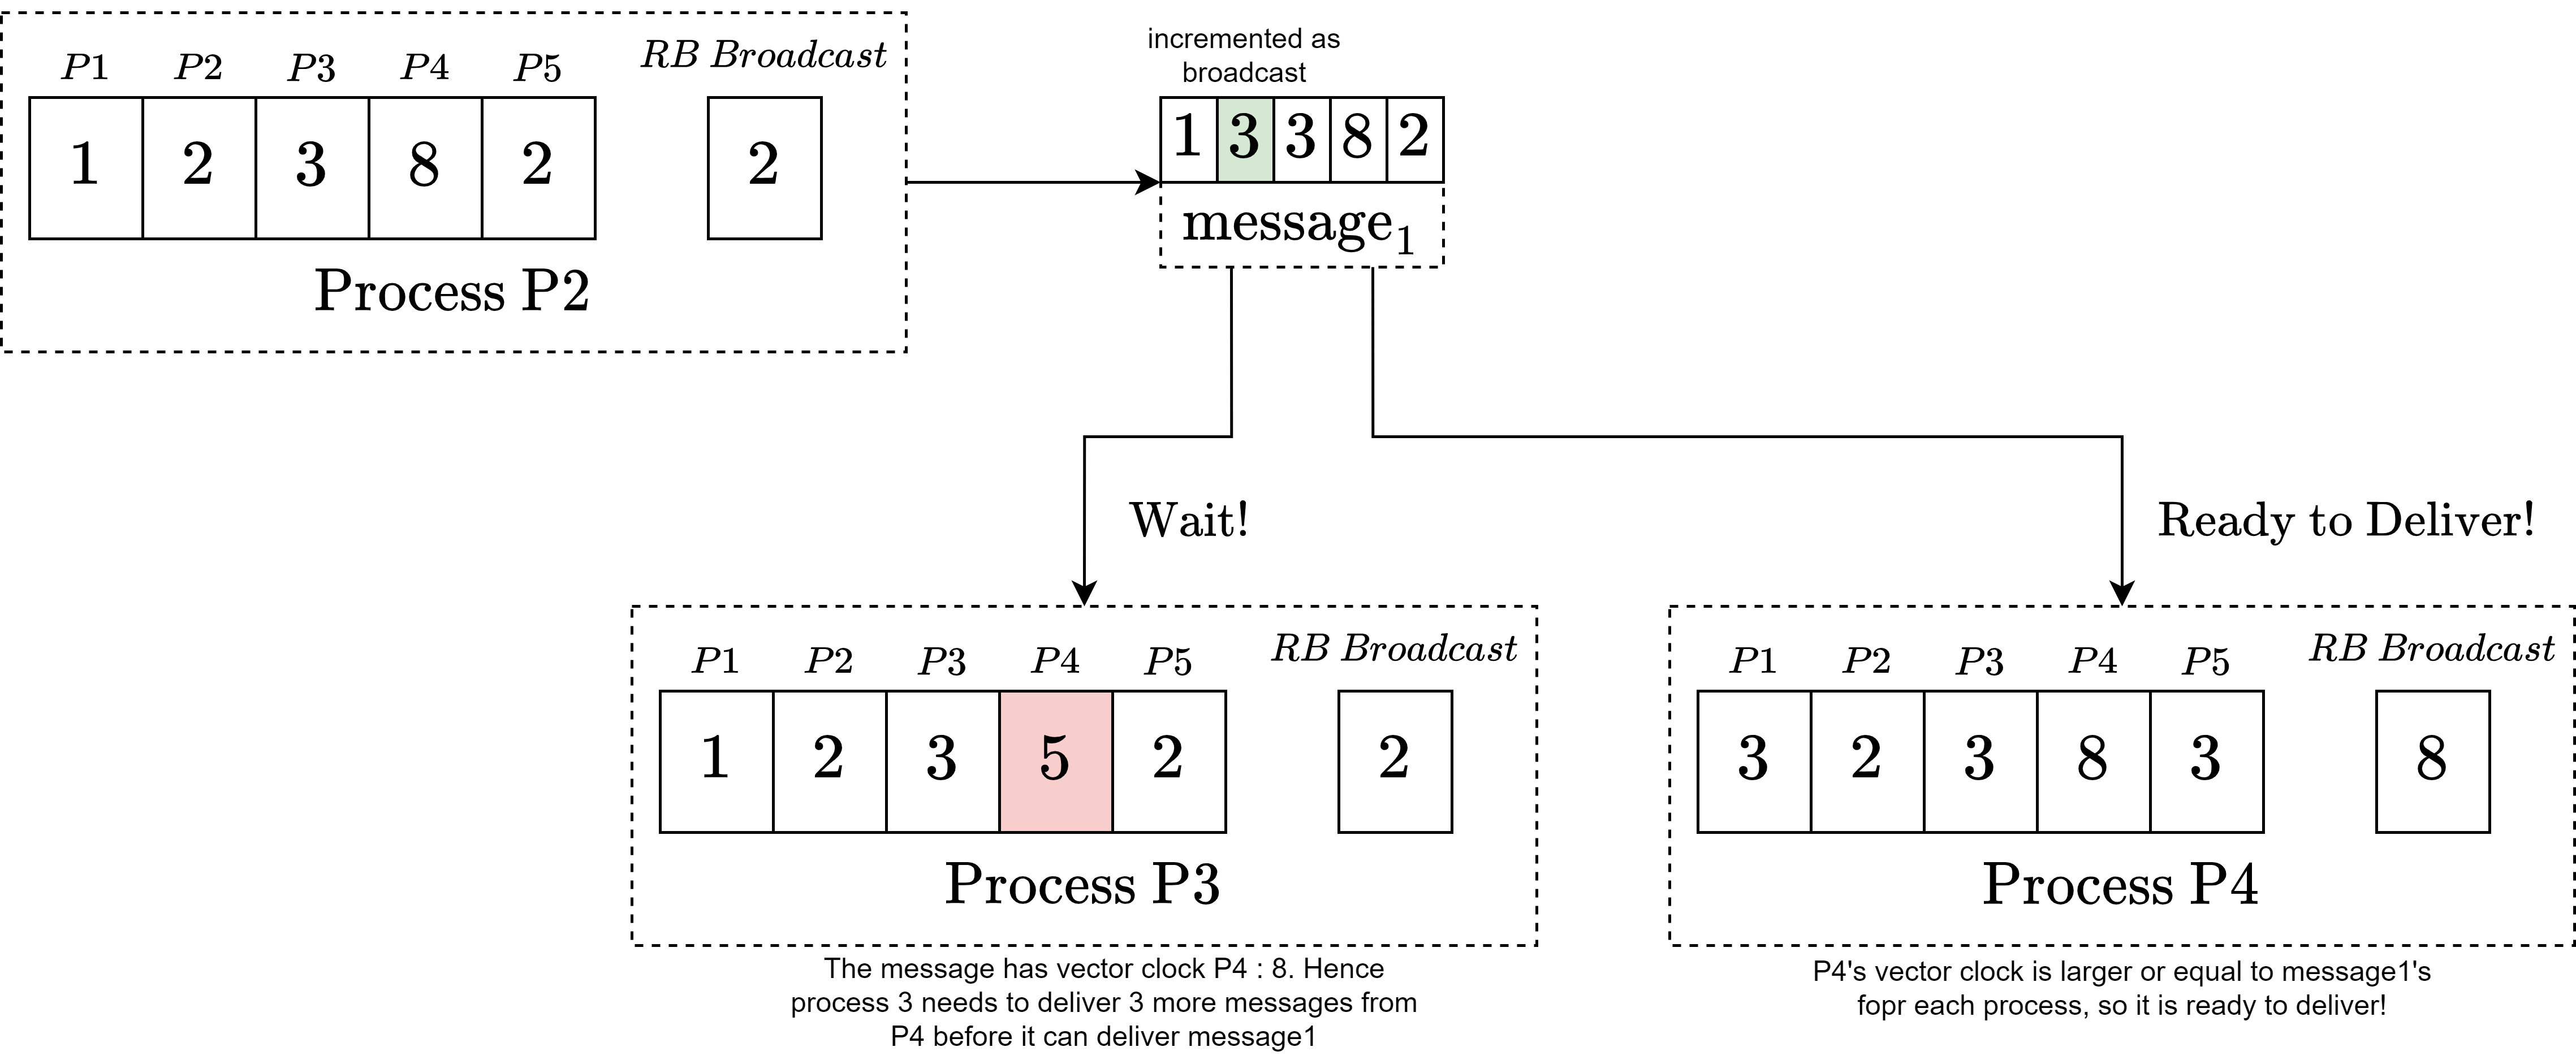
\includegraphics[width=.9\textwidth]{broadcast/images/causal_broadcast_vector_clocks.drawio.png}
\end{center}
\inputminted{elixir}{broadcast/code/causal_reliable_broadcast_vector_clock.ex}

\subsection{Total Order Message Delivery}
\begin{definitionbox}{Total Order/TO Message Delivery}
    All correct messages deliver the same global order of messages.
    \begin{itemize}
        \item Impossible in an asynchronous system as there is no shared clock, so no way to determine a shared ordering. 
        \item Does not need to be \textit{FIFO} but is usually implemented so.
        \item Sometimes called \textit{atomic broadcast}.
    \end{itemize}
    \begin{center}
        \begin{tabular}{l l p{.6\textwidth}}
            \textbf{Uniform Total Order} & Safety & If a correct or crashed process delivers $M_1 \prec M_2$, then no correct process delivers $M_2 \prec M_1$. \\
            \multicolumn{3}{c}{\textbf{All Properties from Uniform Reliable Broadcast}} \\
        \end{tabular}
    \end{center}
    In order to have a total order, processes must reach a consensus on the global order.
\end{definitionbox}
